\section{Strømforsyning}\label{sec:car_psu} %Please start this section on a left page

For at dimensionere strømforsyningen er der i første omgang udarbejdet et estimat for hvor meget strøm de forskellige blokke i bilen forbruger.
Resultater af disse udregninger er indsat i tabel \ref{tbl:bil_forsyninger} på side \pageref{tbl:bil_forsyninger}.
Generelt kan det siges at de forskellige udgange er dimensioneret efter forbrugere på bilen, dette inkluderer en Raspberry Pi 2, et PSoC4 Pioneer Kit samt diverse sensorer.
Det noteres at PSoC4 Pioneer Kit ikke blev taget med i betragtning under designet af strømforsyningen, da denne er blevet tilføjet til projektet meget sent i forløbet.

Strømforsyningen er som udgangspunkt designet som en buck converter \cite[afsnit 6.10]{lib:analogteknik}.
Til at realisere dette er en TI LM26003 taget i brug som central enhed.
I databladet for LM26003\cite{lib:lm26003} fremgår et typisk design, som stemmer godt overens med behovene for dette projekt.

Til selve dimensioneringen af kredsløbet er fremgangsmåden, der fremkommer i databladets punkt 9.2.1 fulgt. 
Der er lavet en mindre modifikation ift. \ref{fig:lm26003fig16}, ''Typical Application'', for at give strømforsyningen en 3V udgang.

\begin{figure}[h]
\centering
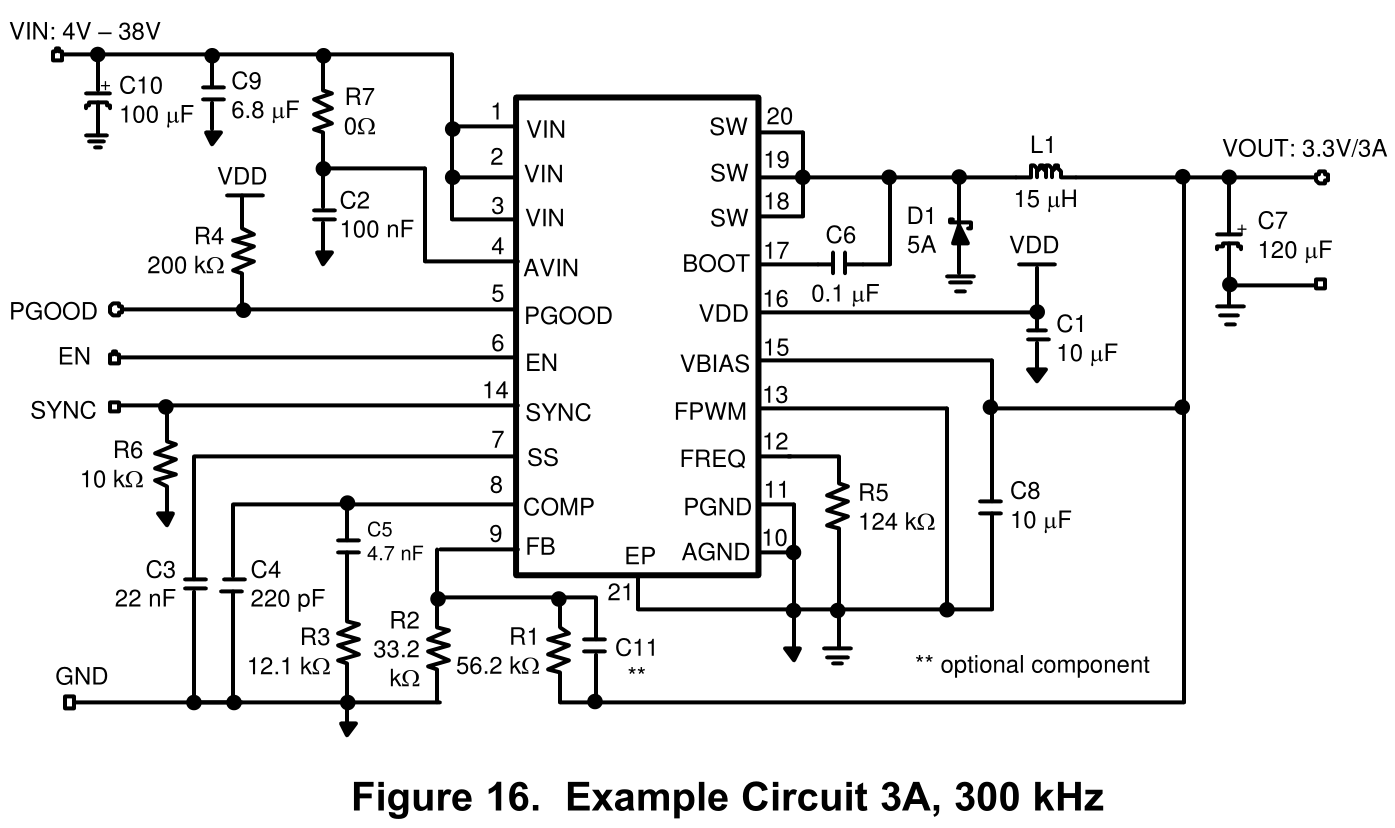
\includegraphics[width=\textwidth* 9/10]{../fig/billeder/lm26003fig16}
\label{fig:lm26003fig16}
\caption{Typisk kredsløb fra databladet for LM26003}
\end{figure}

I forbindelse med L1 er der på samme kerne viklet viklinger på for at danne en transformer, hvorved en 3V udgang er lavet. 
Denne ensrettes med en diode og filtreres med en kondensator. 

U2 på figur \ref{fig:bil_psu} består af den føromtalte egenviklede transformer, som er viklet på en axial spoleform. 
Denne kan ses i databladet for den anvendte spolekerne\cite{lib:psu_L1core}. 
Samtlige beregninger for strømforsyningen fremgår i bilaget\cite{lib:psu_calcs}.
For at overholde kravene om en lav ESR, ækvivalent seriemodstand, for kondensatorerne C1, C9 og C10 er disse bestilt udefra, da de elektrolytkondensatorer, som forefindes på skolens komponentlager har langt for høj ESR. 
En for høj ESR vil medføre at polen for det pågældende lavpasfilter lægges for langt ned i frekvens til at fjerne dynamikken i det pågældende signal.

Samtlige udregninger i forbindelse med design af strømforsyningen findes i projektets bilag\cite{lib:psu_calcs}.

\begin{landscape}
\begin{figure}[h]
\centering
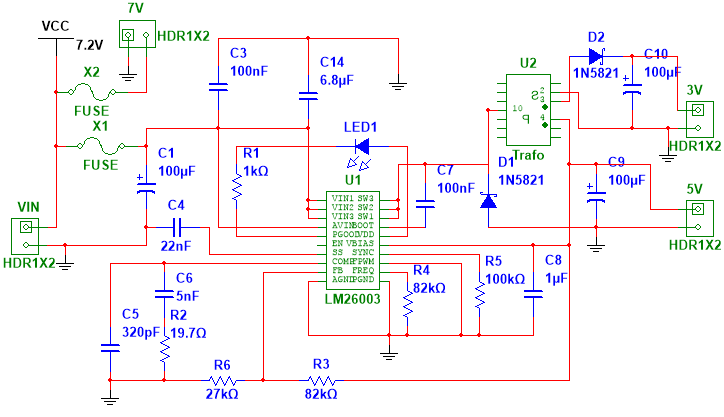
\includegraphics[height=\textwidth-3.5 cm]{../fig/diagrammer/bil/psu_kredsloeb}
\caption{Kredsløbsdiagram for strømforsyning i bilen}
\label{fig:bil_psu}
\end{figure}
\end{landscape}